%**************************************************************
\section{Confronto fra la precedente app e quella nuova}
\label{sec:confronto-precedente-app-nuova}

In questa sezione vengono mostrate le differenze più significative fra la precedente app (in uso presso l'azienda) e quella nuova, realizzata durante lo stage.\\
Queste differenze sono dovute principalmente alla richiesta da parte del tutor aziendale di pensare a come poter fare un restyling grafico dell'applicazione che attualmente hanno in uso.
Quest'ultima infatti, essendo un po' datata, è stata progettata con un impianto grafico e con un'esperienza utente diverse da quelle da quelle attuali.\\
Innanzitutto, gli schermi degli smartphone e dei tablet sono, negli ultimi anni, diventati sempre più grandi e con risoluzioni più elevate, offrendo più spazio per disporre il contenuto di una schermata.
Non ha quindi più senso, ad esempio, avere liste scorrevoli di elementi che sono condensate. Ci si può permettere di spaziare molto di più gli elementi e anche migliorare anche lo spazio fra una linea di testo e un'altra.\\
Inoltre, entrambi i sistemi operativi per cui sviluppare l'applicazione hanno un loro stile grafico, per cui va valutato se creare due interfacce utenti del tutto simili ma con componenti che ricalcano quelle native oppure cercare di creare un'interfaccia che possa andare bene per entrambe, evitando di utilizzare componenti grafiche specifiche per l'uno o per l'altro sistema.
Ad esempio, nel \emph{Material Design} di Google vi sono delle componenti chiamate \emph{Floating Action Button} (dei pulsanti a forma circolare posizionati solitamente in basso al centro/destra che "fluttuano" sopra il contenuto), da utilizzare come pulsanti per svolgere azioni come la modifica di contenuti testuali, che in Android si integrerebbero correttamente, in iOS invece no.\\
Un'altra riflessione che è stata fatta è relativa ai menu principale dell'applicazione: come viene mostrato in "\hyperref[subsec:menu-applicazione]{Menu dell'applicazione}", difficilmente viene ancora usato un menu a tendina per mostrare funzionalità secondarie, preferendo invece un menu di tipo "drawer".\\
Altre considerazioni e dimostrazione dei miglioramenti apportati si possono trovare nelle sotto-sezioni che seguono.

% \clearpage % Tenere se non viene scritto altro in questa sezione.

%**************************************************************
\subsection{Informazioni sull'applicazione}
\label{subsec:informazioni-applicazione}

Questa schermata è disponibile aprendo il menu dell'applicazione (schermata che viene presentata in seguito a questa) e mostra informazioni generali sull'applicazione, tra cui il server a cui si è connessi, il nome utente e la versione.\\
Il contenuto di questa schermata, che nella app dell'azienda è condensato verso l'alto, viene ora reso più spaziato e inserito in più elementi di una lista scorrevole permettendo, in futuro, di aggiungere contenuti alla schermata senza problemi.\\
I due loghi, dell'azienda presso cui si è svolto lo stage e dell'azienda di cui è partner, sono stati resi cliccabili ed entrambi reindirizzano al rispettivo sito web.

\begin{figure}[!h]
  \centering 
  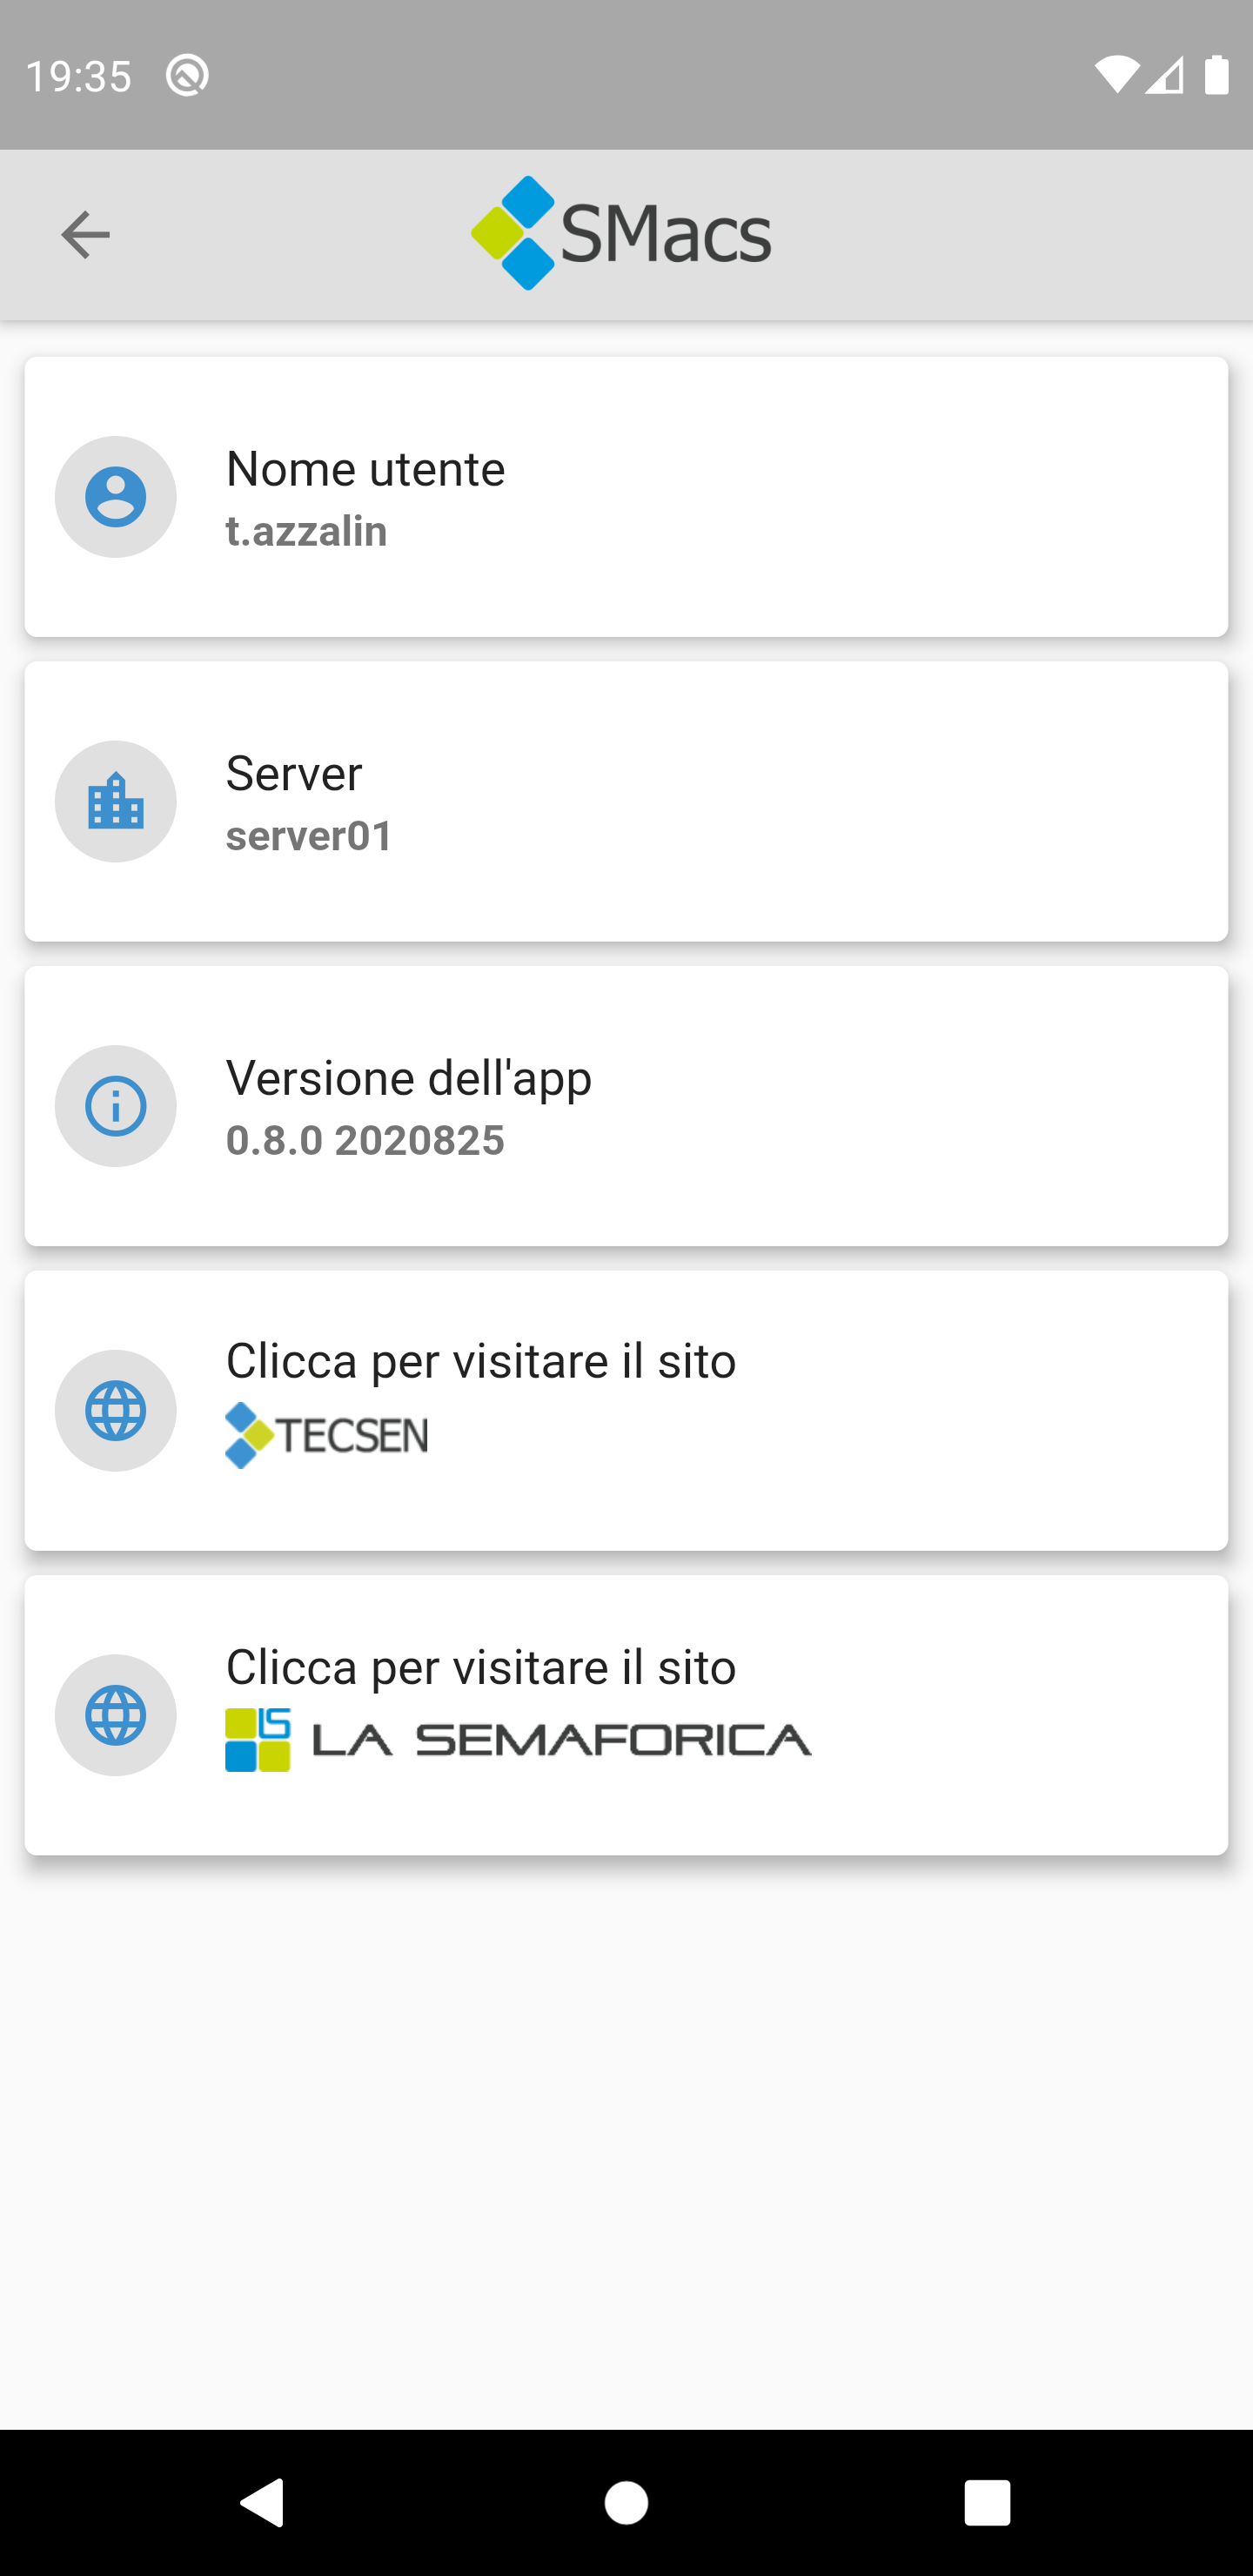
\includegraphics[width=0.75\columnwidth]{capitolo-6/confronto-app-vecchia-nuova/AppInfoView} 
  \caption{Confronto fra schermate delle app: Informazioni sull'applicazione}
\end{figure}

\clearpage % Tenere per assicurarsi che ci sia un'immagine per pagina e basta.

%**************************************************************
\subsection{Menu dell'applicazione}
\label{subsec:menu-applicazione}

Il menu dell'applicazione è accessibile, così come nell'app dell'azienda, solamente attraverso la schermata della lista degli impianti.\\
Prima disponibile sotto forma di menu a tendina, nella versione realizzata per lo stage è stato realizzato un menu di tipo \emph{drawer} (dall'inglese, cassetto, perché alla richiesta di apertura effettua una transizione dall'esterno all'interno e si richiude in maniera inversa), che appare da sinistra alla pressione del pulsante \emph{hamburger} (il pulsante con tre linee parallele orizzontali è stato così ribattezzato perché assomiglia ad un panino di un fast food) in alto a sinistra (visibile nella schermata di destra nell'immagine sottostante).\\
Le voci del menu sono state mantenute così com'erano ad eccezione della voce "Refresh", che aggiorna la lista di impianti disponibile localmente riscaricandola dai server aziendali, che è stata rimossa in favore di un più accessibile pulsante presente direttamente nella barra di navigazione in alto alla schermata, riducendo il numero di click necessari per raggiungerlo.

\begin{figure}[!h]
  \centering 
  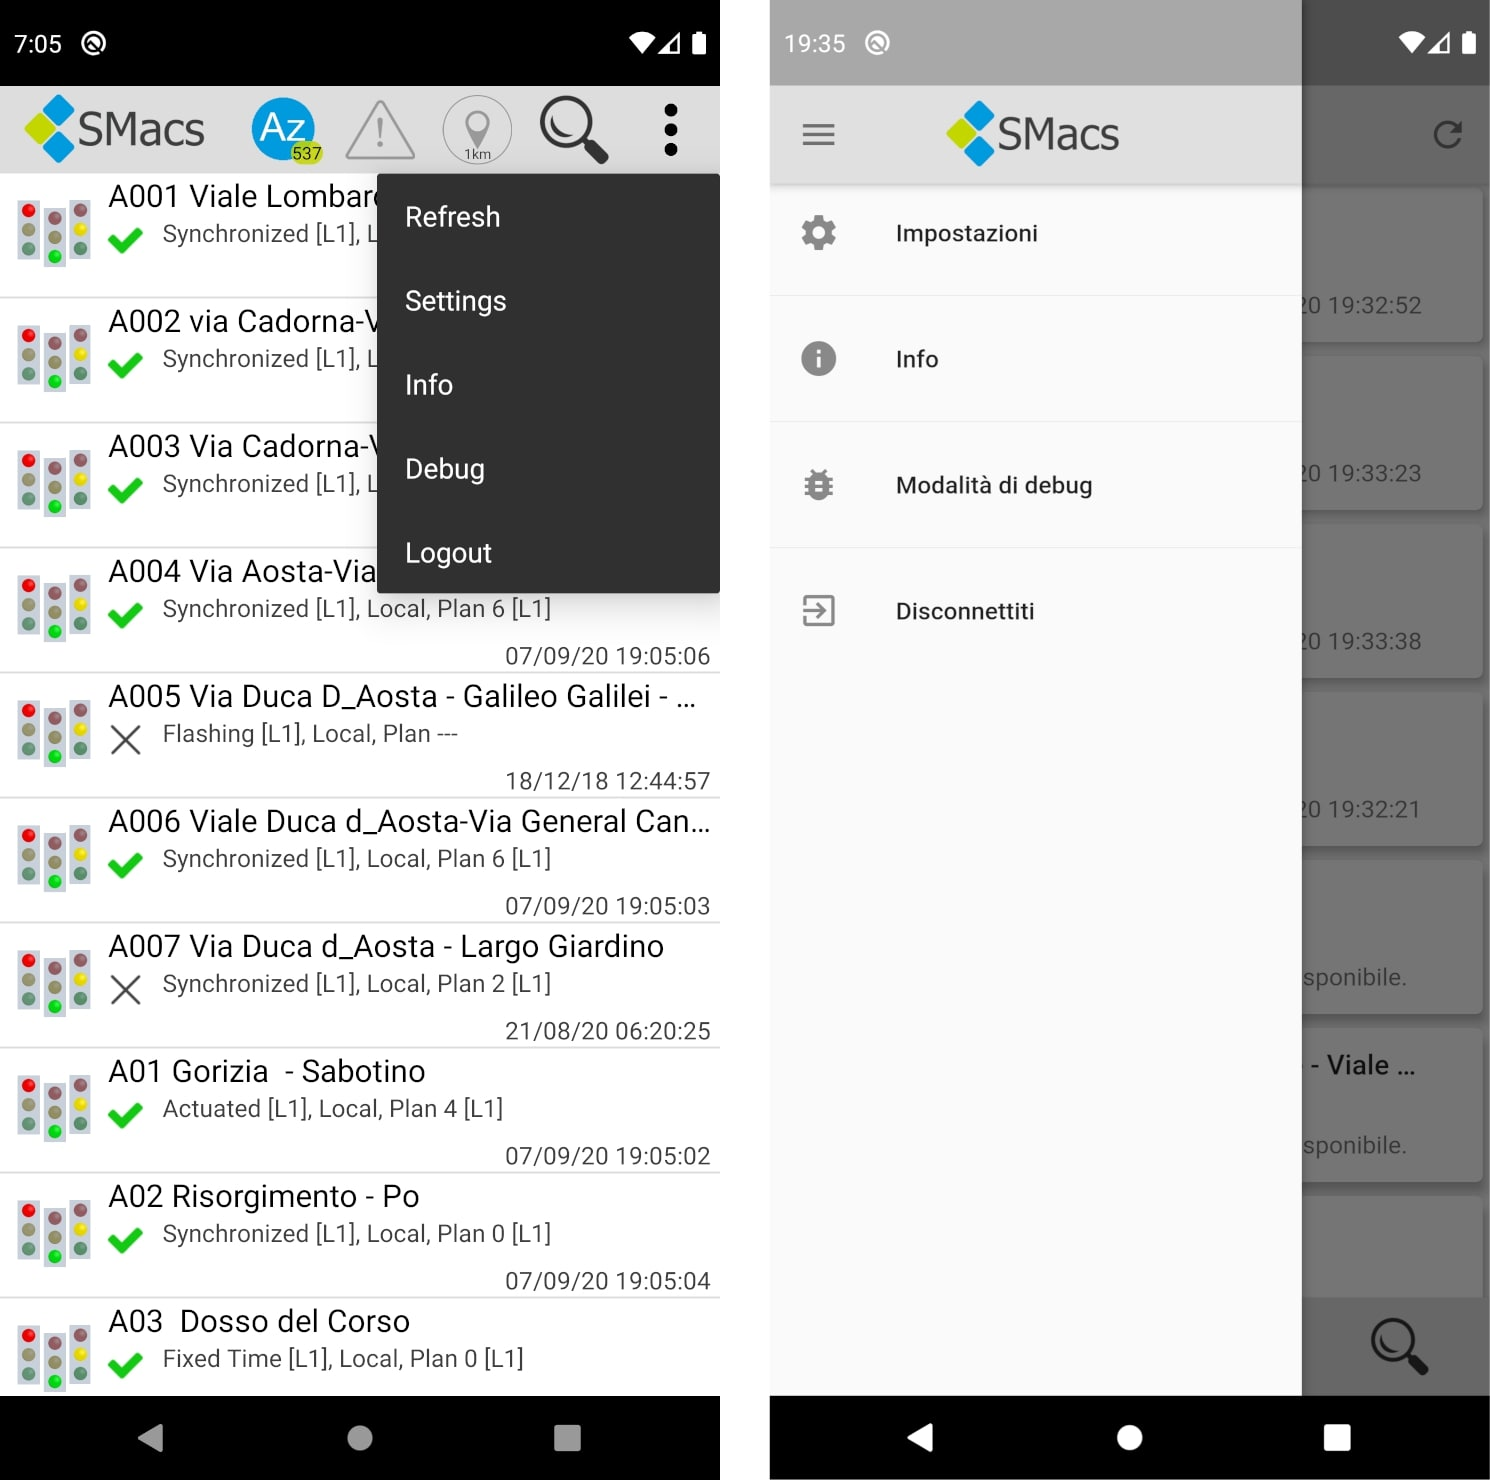
\includegraphics[width=1.0\columnwidth]{capitolo-6/confronto-app-vecchia-nuova/DrawerView} 
  \caption{Confronto fra schermate delle app: Menu dell'applicazione}
\end{figure}

\clearpage % Tenere per assicurarsi che ci sia un'immagine per pagina e basta.

%**************************************************************
\subsection{Lista degli impianti}
\label{subsec:lista-impianti}

La schermata in cui viene mostrata la lista degli impianti è rimasta sostanzialmente invariata se non per alcune modifiche prettamente estetiche.\\
I pulsanti per filtrare la lista sono stati spostati dalla barra di navigazione in alto a una barra apposita in basso e, come è stato detto in precedenza, il pulsante di "Refresh" è stato estratto dal menu per averlo disponibile nella barra di navigazione.\\
A differenza dell'applicazione in uso presso l'azienda, non tutte le funzionalità sono disponibili: tutti gli elementi della lista la cui icone rappresentano dei semafori sono cliccabili (e portano alla schermata di dettaglio) mentre gli altri, come i primi due elementi della lista della schermata di destra, non lo sono.\\
In quest'ultimo caso, la pressione dell'elemento visualizza un avviso all'utente che lo informa sul fatto che la funzionalità non è ancora disponibile.

\begin{figure}[!h]
  \centering 
  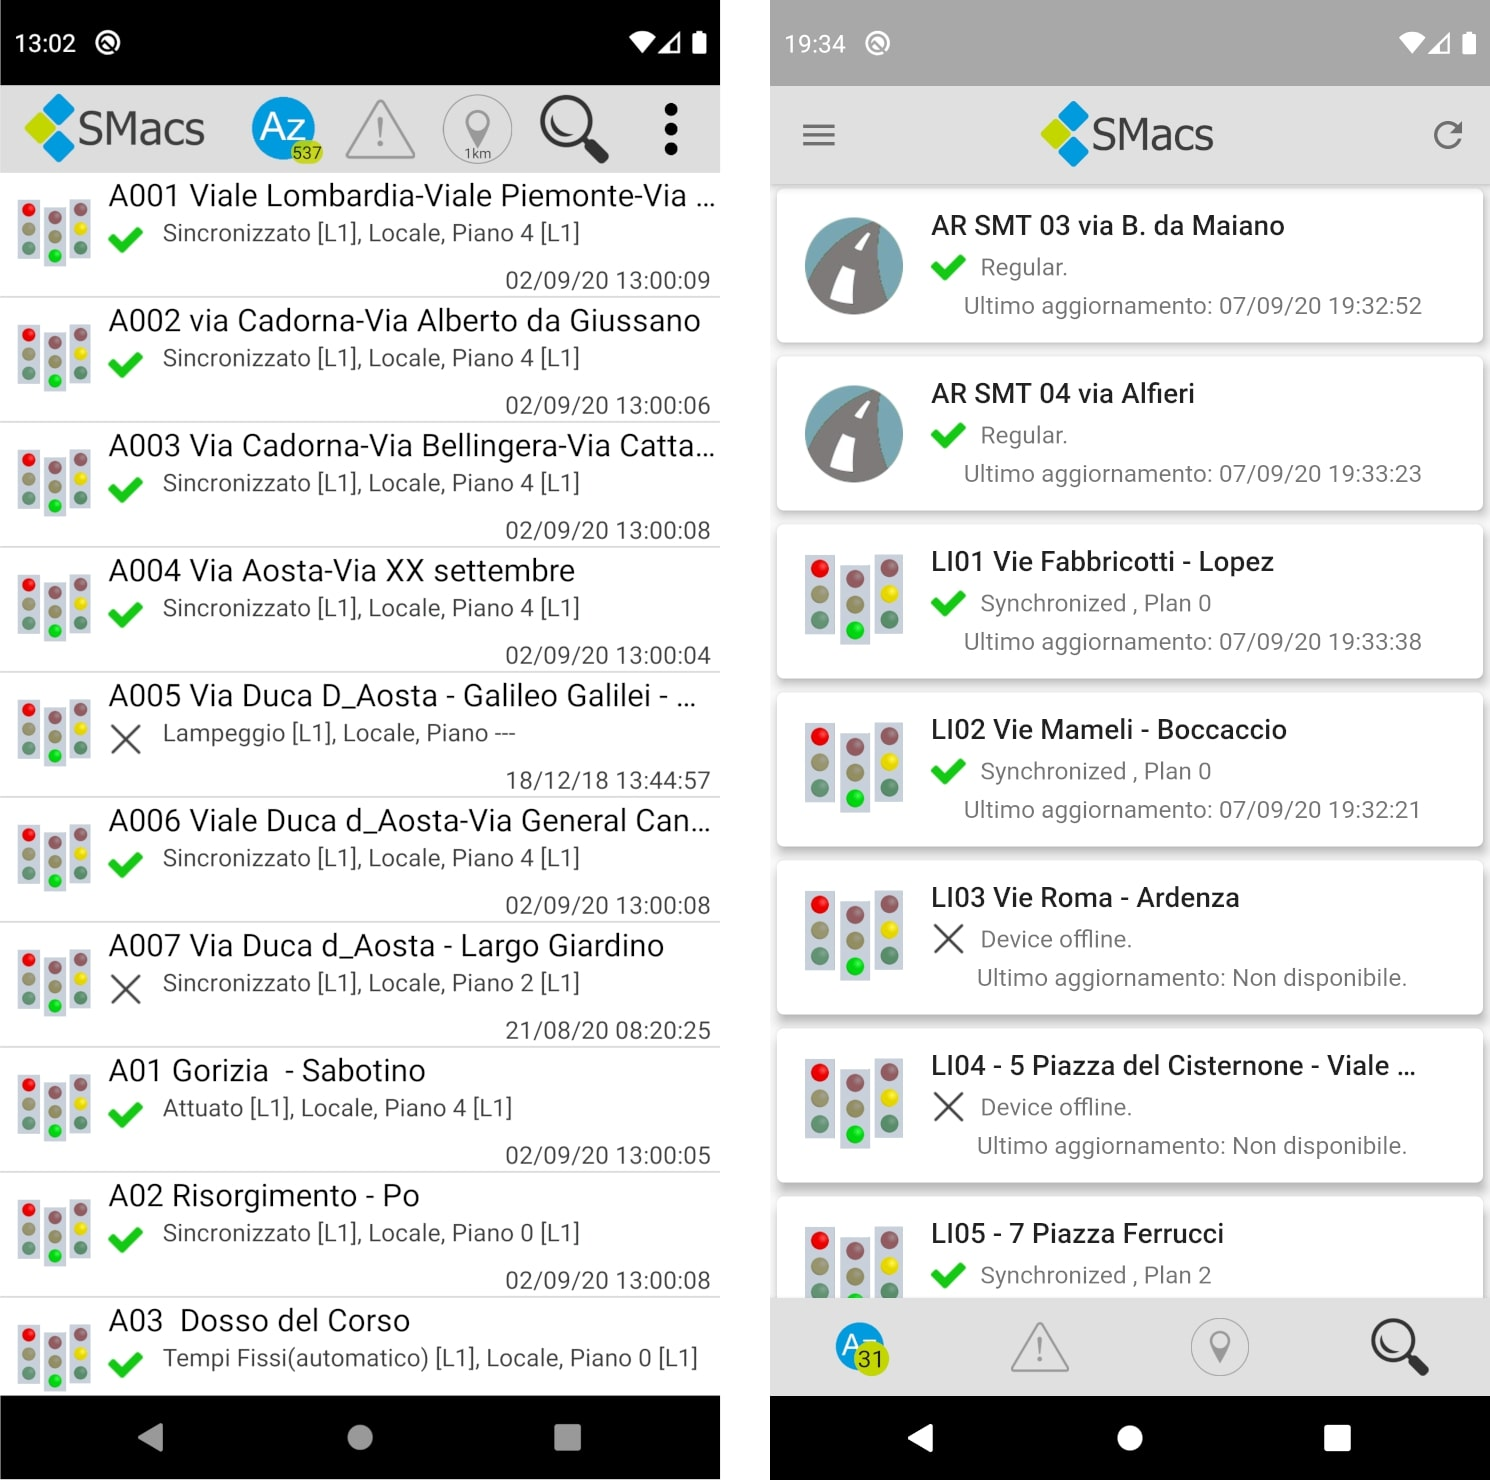
\includegraphics[width=1.0\columnwidth]{capitolo-6/confronto-app-vecchia-nuova/DeviceListView} 
  \caption{Confronto fra schermate delle app: Lista degli impianti}
\end{figure}

\clearpage % Tenere per assicurarsi che ci sia un'immagine per pagina e basta.

%**************************************************************
\subsection{Pannello di controllo}
\label{subsec:pannello-controllo}

La schermata del dettaglio di un regolatore semaforico è cambiata sensibilmente.\\
Questa schermata comprende tutta ciò che è presente nell'immagine di destra, incluse le tre schede "Panoramica", "Diagnostica", "Pannello di controllo" e il loro contenuto.
Dalla pulsantiera in basso sono stati rimossi il "Pannello di controllo", che è appunto diventata una scheda, e il pulsante "Indicazioni stradali", giustificato dal fatto che premendo il pulsante "Posizione" si apre l'applicazione di mappe del dispositivo, che già propone l'avvio nella navigazione.\\
È stato invece inserito il pulsante "Info" che rimanda alla schermata con le informazioni dell'hardware e del software del regolatore semaforico.\\
Oltre a queste modifiche, che sono comuni a "Panoramica" e a "Diagnostica", nella schermata "Pannello di controllo" è stata semplificata l'interfaccia, rendendola più simile a quella attualmente usata negli applicativi per desktop dell'azienda (a fini di unificazione dell'esperienza utente).
In particolare, la pulsantiera "Funzione" è diventata un menu a tendina, "Reset allarmi" è stata spostata nella scheda "Diagnostica" e le altre funzionalità è stato chiesto di non inserirle.

\begin{figure}[!h]
  \centering 
  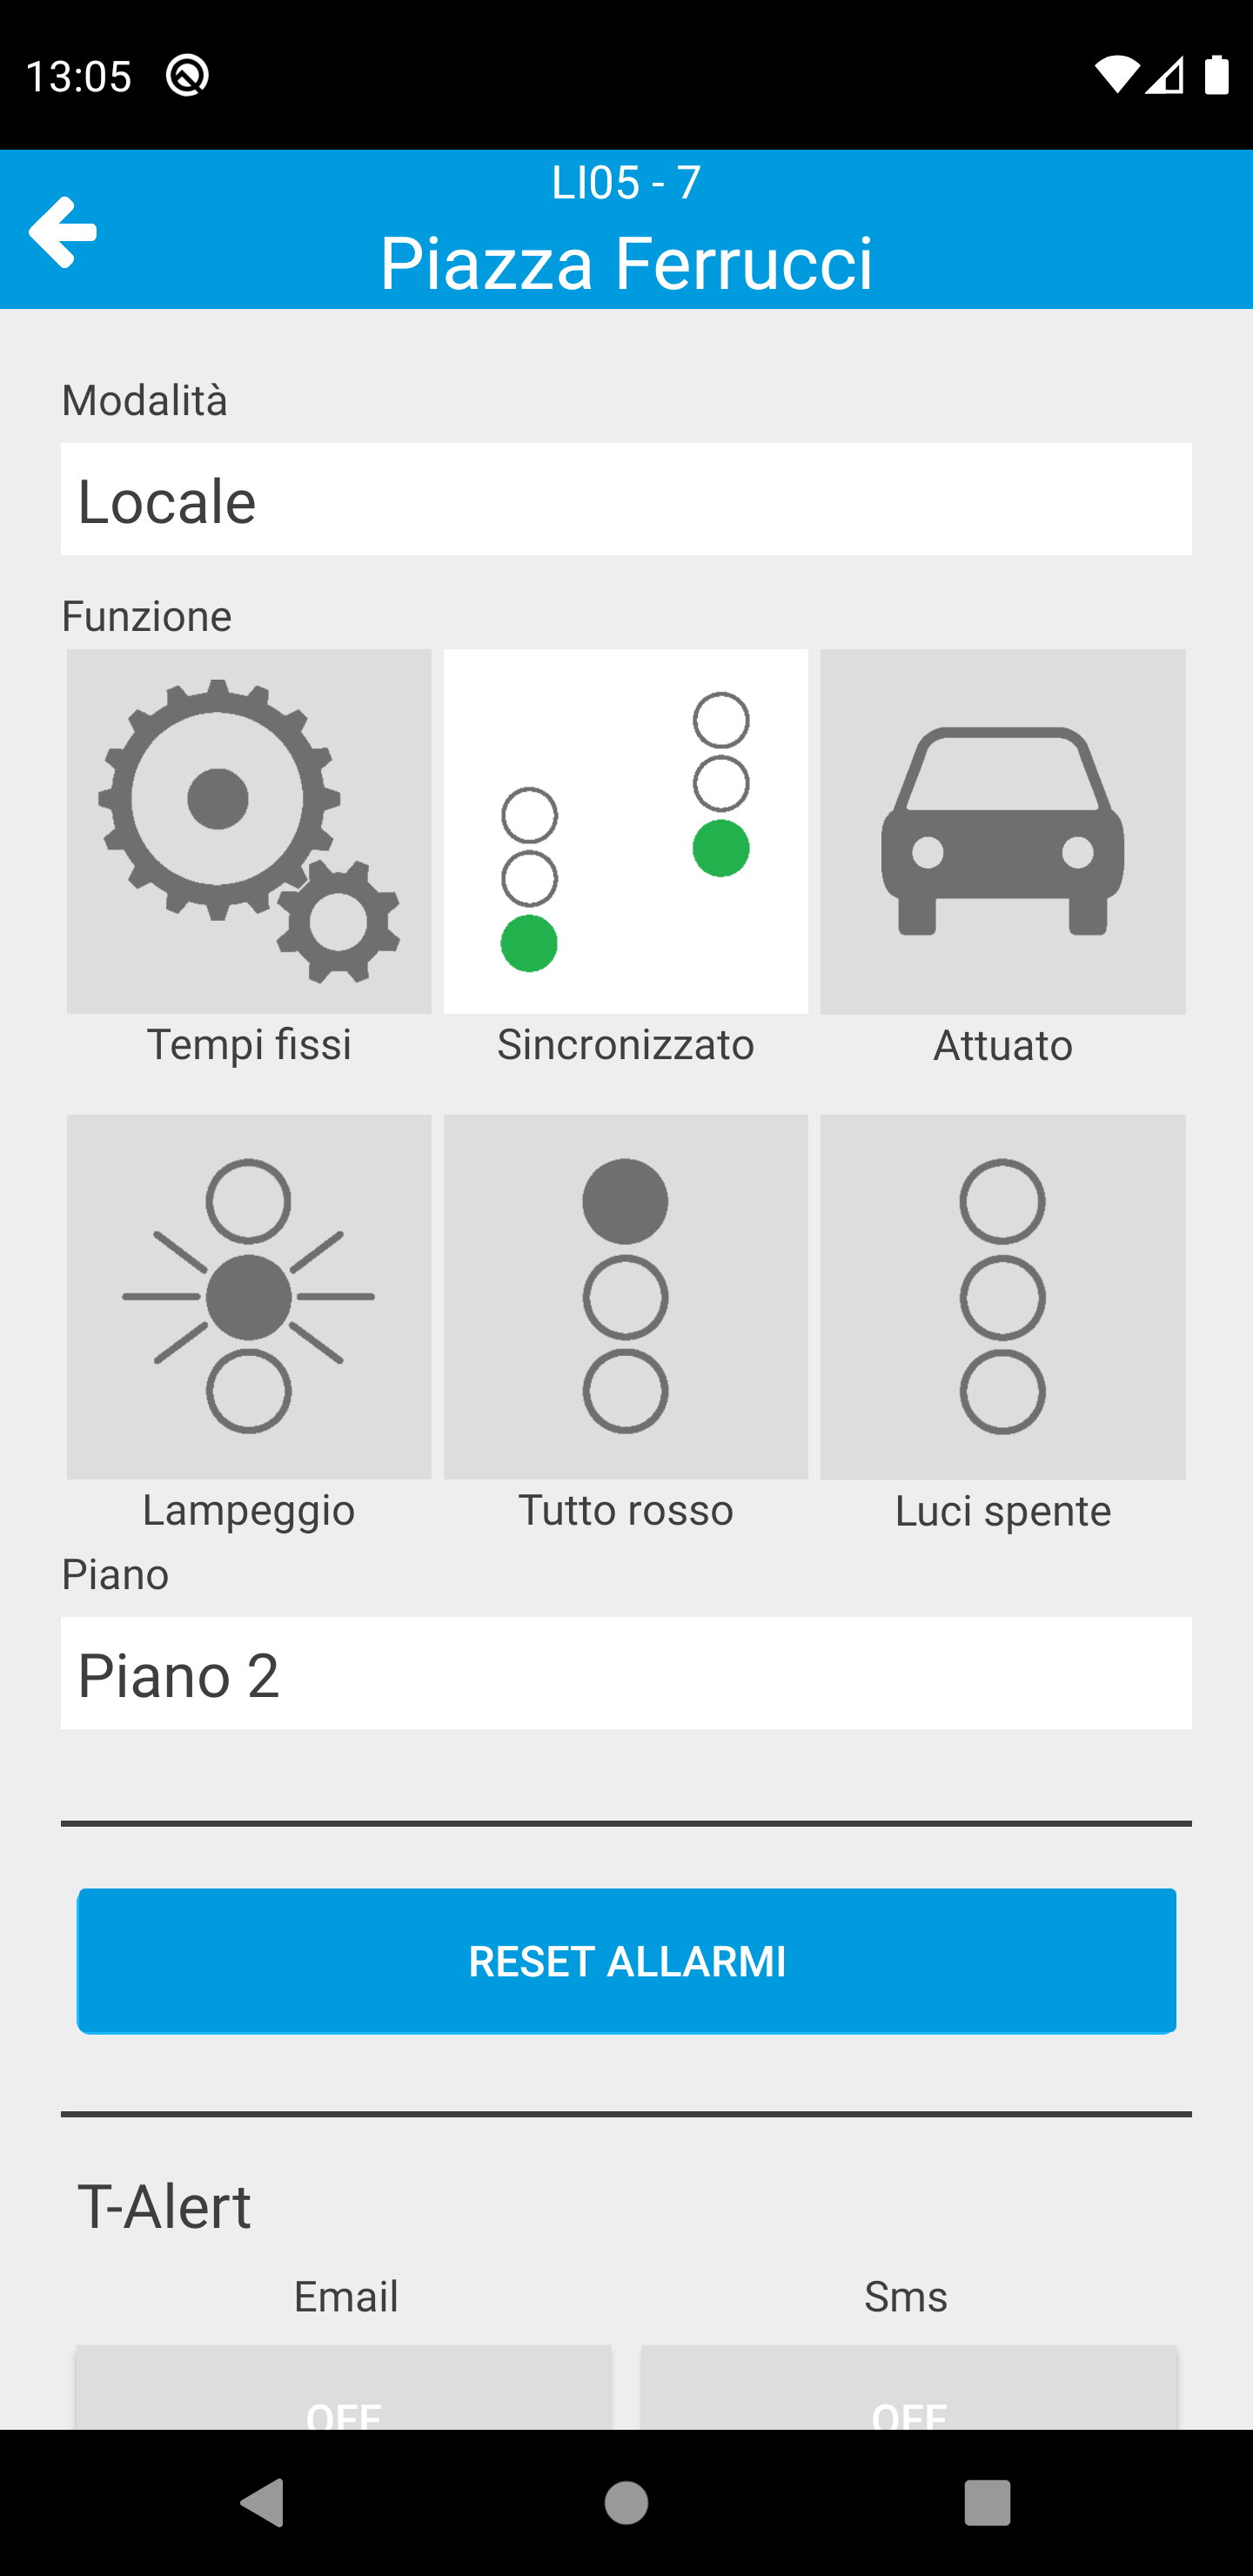
\includegraphics[width=1.0\columnwidth]{capitolo-6/confronto-app-vecchia-nuova/ControlPanelView} 
  \caption{Confronto fra schermate delle app: Pannello di controllo}
\end{figure}

\clearpage % Tenere per assicurarsi che ci sia un'immagine per pagina e basta.

%**************************************************************
\subsection{Panoramica sull'impianto}
\label{subsec:panoramica-impianto}

Come precedentemente affermato, la schermata del dettaglio è cambiata sensibilmente.\\
Dopo aver elencato i cambiamenti avvenuti nella scheda "Pannello di controllo" e nella pulsantiera in basso alla schermata, possiamo notare come tutte le icone di semafori e degli input (le icone sottostanti) siano state rimosse e le informazioni testuali semplificate.\\
Le icone appena citate sono state rimosse perché rappresentano le stesse che sono posizionate sopra l'immagine dell'intersezione stradale nella schermata di destra.
Questa funzionalità di visione dell'intersezione è chiamata \emph{sinottico} ed è disponibile attualmente nell'app aziendale previa pressione del pulsante a forma di intersezione stradale, situato accanto all'icona di aggiornamento, in alto a destra della schermata di sinistra.\\
Infine, la lista dei messaggi di diagnostica (nell'immagine di sinistra, quella che parte dal centro, sotto la scritta "Dettagli - 1 Info") è stata spostata nella scheda "Diagnostica".

\begin{figure}[!h]
  \centering 
  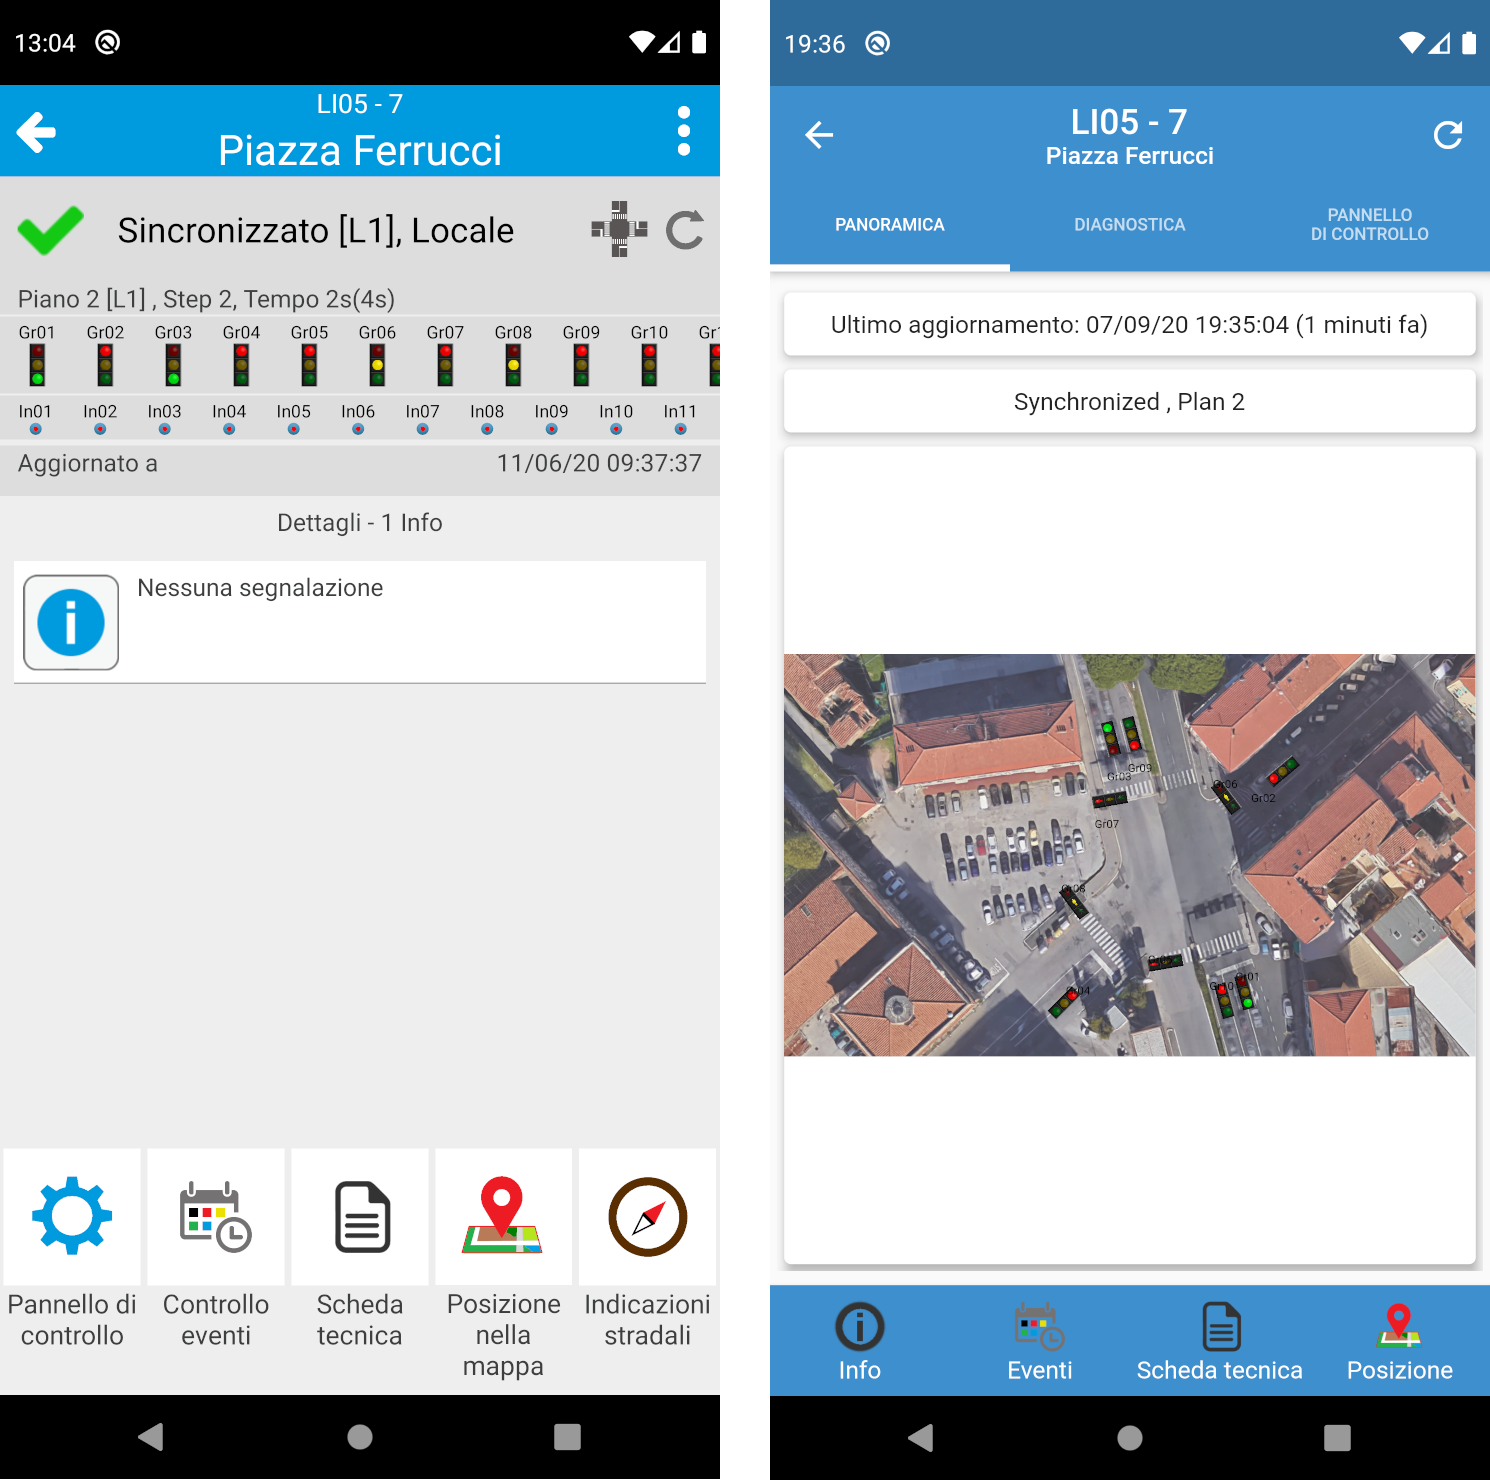
\includegraphics[width=1.0\columnwidth]{capitolo-6/confronto-app-vecchia-nuova/DeviceOverviewView} 
  \caption{Confronto fra schermate delle app: Panoramica sull'impianto}
\end{figure}